\chapter{Draaiveld}
We weten nu dus dat we een statorveld hebben, we gaan nu kijken naar hoe we deze gaan
opwekken en hoe we dit kunnen gebruiken om een rotor te laten draaien.
Even ter verduidelijking ook, de rotor heeft dus ook een magnetisch veld en dat was degene
met een constant magnetisch veld, maar de stator heeft een \textbf{draaiveld} (rotating
field).
Dit is een magnetisch veld dat in de ruimte draait.

\begin{figure}[H]
  \centering
  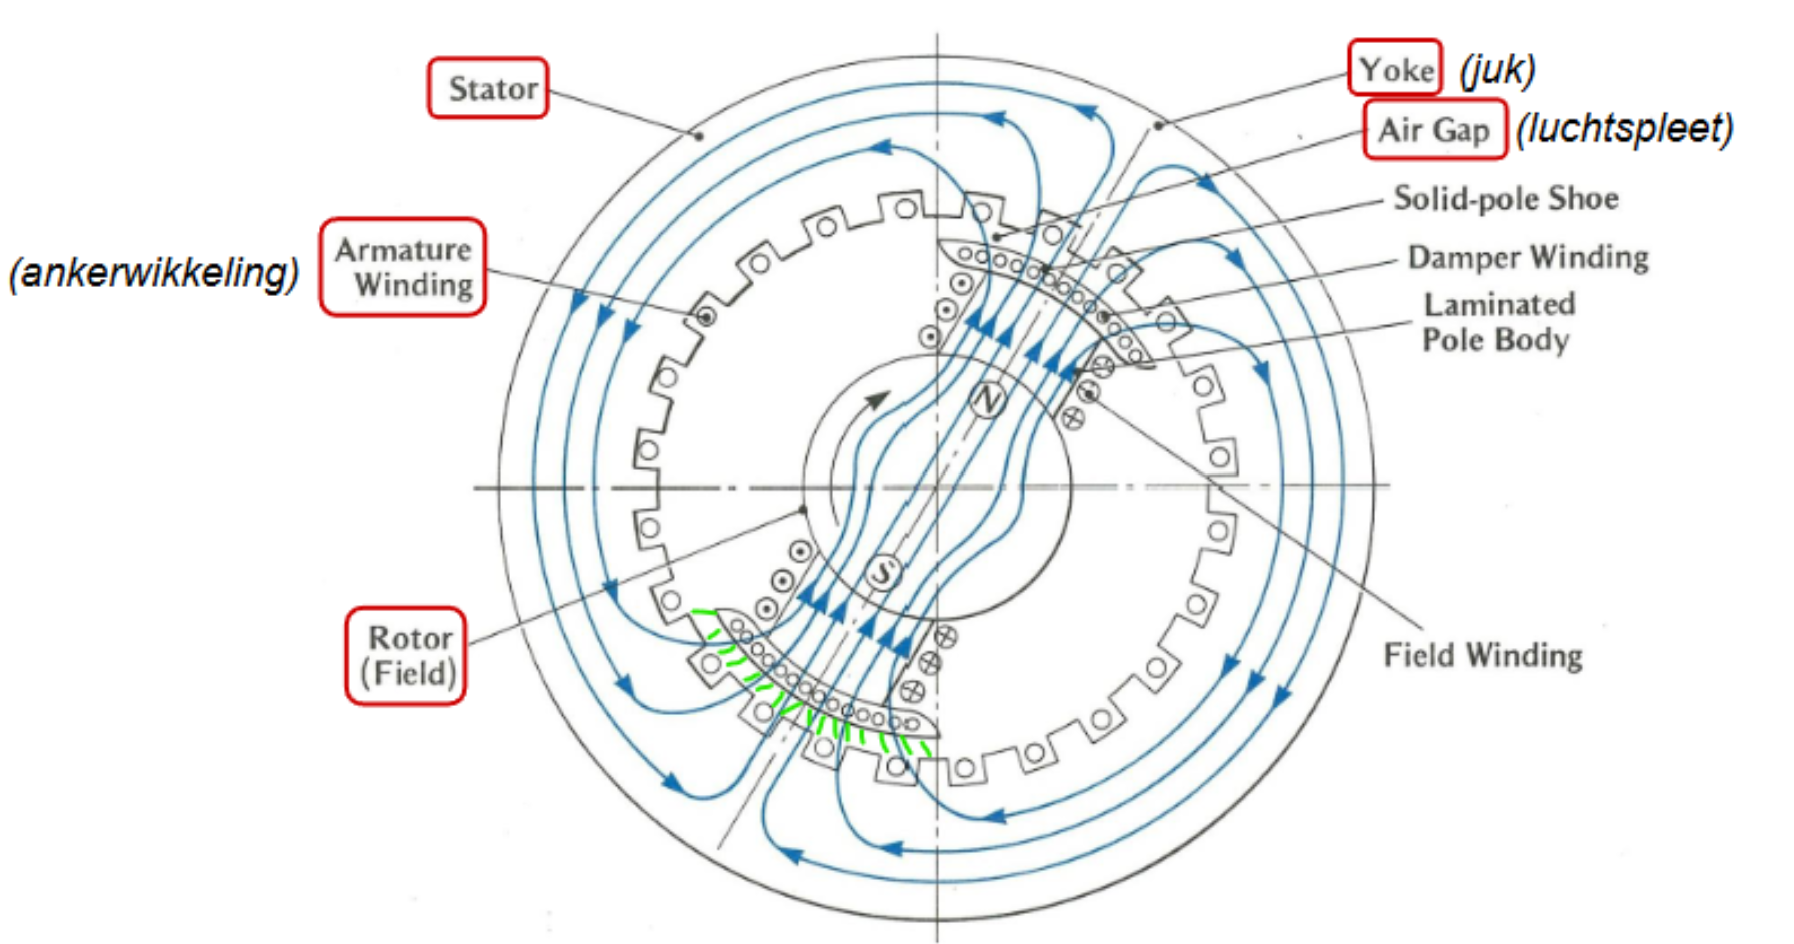
\includegraphics[width=0.7\textwidth]{assets/weergavemagnetischveldinmotor.png}
  \caption{Magnetisch veld in een motor}
  \label{fig:weergavemagnetischveldinmotor.png}
 \end{figure}

Tussen de stator en de rotor is er dus een \textbf{luchtspleet}, typisch 0,5 tot 1mm
groot, in de figuur hierboven is deels van die luchtspleet aangeduid in het groen.
Het magnetisch veld van de stator gaat hierdoor om tot de rotor te geraken en het rotor
veld het stator veld te doen volgen maar dit zien we zometeen.
De 'Yoke' of \textbf{juk} is waar de veldlijnen 'terugkeren' langs de achterkant, wat je
je een beetje kan inbeelden door naar deze figuur te zien.

We veronderstellen nu dat onze rotor een mooie ronde ijzeren cilinder is, dit maakt het
meer symmetrisch en maakt dat onze analyse die we nu gaan doen volledig correct is.
We kijken even naar 1 van die wikkelingen, deze is dan gesitueerd in die statorgleuven
zoals in de volgende figuur:

\begin{figure}[H]
  \centering
  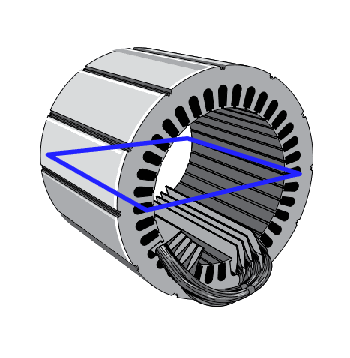
\includegraphics[width=0.4\textwidth]{assets/1wikkelinginstator.png}
  \caption{1 wikkeling in stator}
  \label{fig:1wikkelinginstator.png}
 \end{figure}

\newpage

Als we nu door deze éne wikkeling een wisselstroom sturen, dan zal er door die wikkeling
ook een wisselveld ontstaan, dit is een magnetisch veld dat in de ruimte oscilleert, op en
neer eigelijk zoals in deze figuur:

\begin{figure}[H]
  \centering
  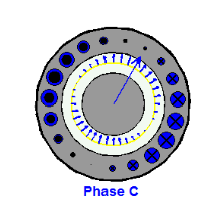
\includegraphics[width=0.4\textwidth]{assets/1wikkelingwisselveld.png}
  \caption{1 wikkeling met wisselveld}
  \label{fig:1wikkelingwisselveld.png}
 \end{figure}

Hier staat het wel een beetje schuin onder een hoek, de animatie hiervan staat gewoon op
toledo je kan die daar bezien.
Die gele lijn is de luchtspleet, het is vanaf hier dat de magnetische veld vectoren
getekend worden.
We zijn vooral geinteresseerd in die luchtspleet want hier gaat het over van stator naar
rotor, zo wordt het koppel opgewekt.
Als we nu 2 andere wikkelingen plaatsen, die elk 120° van elkaar verwijderd zijn, en we
sturen door elk van deze wikkelingen een wisselstroom die 120° van elkaar verschoven is,
dan zal er een \textbf{draaiveld} ontstaan.

\begin{figure}[H]
  \centering
  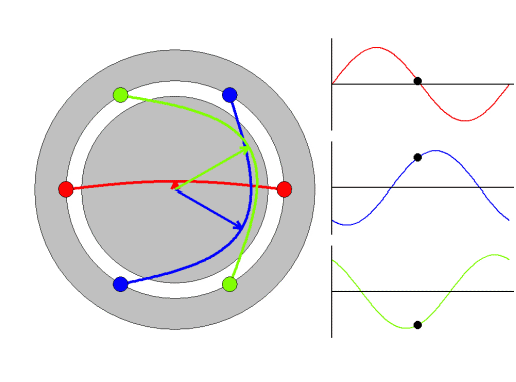
\includegraphics[width=0.5\textwidth]{assets/draaiveld3wikkelingen.png}
  \caption{Draaiveld met 3 wikkelingen}
  \label{fig:draaiveld3wikkelingen.png}
 \end{figure}

Dit is dus ook eigelijk een animatie, waarin die linkse figuur eigelijk die golven alle 3
op en neer gaan en het doet lijken dat het draait (dat doet het ook), check gewoon op
toledo naar deze animatie als je het niet snapt.
Dit kan ook zo weergegeven worden, hierbij draait die roze pijl gewoon tegenwijzerzin,
heel die figuur eigelijk, voor de rest veranderd er niks:

\begin{figure}[H]
  \centering
  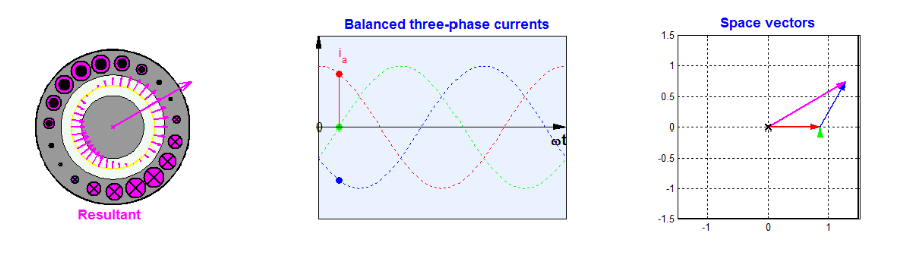
\includegraphics[width=0.8\textwidth]{assets/resulterendedraaiveld.png}
  \caption{Resulterend draaiveld}
  \label{fig:resulterendedraaiveld.png}
 \end{figure}

% Inhoud volgt
Zo een stroom zorgt dus voor een wisselveld, we kunnen deze 3 wisselvelden beschrijven
afhankelijk van hun \textbf{hoekpositie} in de ruimte en hun \textbf{tijdspositie
(faseverschuiving)}, deze gaan in de vorm van de uitdrukking van de \textbf{staande golf}
staan:
\begin{align*}
    B_a(t, \alpha) = \hat{B}_{a} \cdot \sin(\omega_s \cdot t) \cdot \cos(\alpha) \\
    B_b(t, \alpha) = \hat{B}_{b} \cdot \sin(\omega_s \cdot t - 2\pi/3) \cdot \cos(\alpha - 2\pi/3) \\
    B_c(t, \alpha) = \hat{B}_{c} \cdot \sin(\omega_s \cdot t - 4\pi/3) \cdot \cos(\alpha - 4\pi/3)
\end{align*}
Het is dat sinus gedeelte dat de faseverschuiving (tijd) voorstelt en het cosinus gedeelte
de hoekpositie (geometrisch).
Het zijn dus ook deze 3 velden die samen het resulterende draaiveld vormen.

\begin{warningbox}[Faseverschuiving tussen die stromen is belangrijk!]
  Als er door die 3 wikkelingen dezelfde stromen met dezelfde faseverschuiving gaan dan
  krijg je een resulterend veld van 0!
  Het is de verschillende faseverschuivingen dat ervoor zorgen dat je resulterend veld
  niet 0 is.
  Ook belangrijk te onthouden is dat het resulterend veld dan \textit{geen} wisselveld is,
  maar een \textit{draaiveld}
\end{warningbox}

Het draaiveld heeft een bepaalde snelheid, de \textbf{pulsatie}, dit is een
\textbf{elektrische snelheid!} Deze wordt gegeven door:
\begin{align*}
    \omega_s = 2 \pi f
\end{align*}
Het toerental in deze elektrische vorm wordt gegeven door:
\begin{align*}
    n_s = 60 \cdot f
\end{align*}
En eigelijk is die $\alpha$ in die uitdrukkingen van hierboven een geometrische
(mechanische) hoekpositie, maar we hebben ook een elektrische hoekpositie $\theta_{se}$,
dit is eigelijk de faseverschuiving.
Het bepalen van deze hoek wordt gedaan met:
\begin{align*}
    \theta_{se} = p \cdot \theta_{sm} = p \cdot \alpha
\end{align*}
Die $\theta_{sm}$ is gewoon die $\alpha$, het kwam gewoon voor in de les dus ik zeg het
maar zodat je niet verward wordt.
Die p is dus het \textbf{poolpaartal}.

\subsection{Poolpaartal}
Wat is nu het poolpaartal effectief?
Wat is de invloed van de hoeveelheid polen?
Dit is belangrijk om naar te zien want deze machines hebben niet gewoon 3 wikkelingen
zoals we eerder zagen, maar hebben in de praktijk meerdere draden dat door de gleuven van
de stator gaan.
En afhankelijk van hoe je deze draden positioneert kan je een bepaald aantal polen
creëren.
In de volgende figuur zie je dat:

\begin{figure}[H]
  \centering
  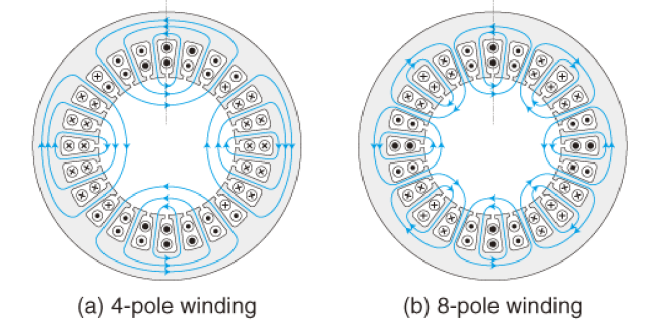
\includegraphics[width=0.6\textwidth]{assets/verschillendepolenevenveeldraden.png}
  \caption{Zelfde constructie met andere polen}
  \label{fig:verschillendepolenevenveeldraden.png}
 \end{figure}

In de industrie gaan we meestal machines met 4 polen (P=4) gebruiken, dus een poolpaartal
p van 2 ($p = \frac{P}{2}$), het poolpaartal is dus het aantal koppels van noord- en
zuidpolen dat een motor heeft.
Hoe meer polen we willen, hoe grotere diameter je echter wel gaat nodig hebben want de
positie van die wikkelingen is voor grotere polen niet voldoende.
Hoe meer polen we hebben hoe lager het toerental van de machine zal zijn, want het
toerental wordt gegeven door:
\begin{align*}
    n_s = \frac{60 \cdot f}{p}
\end{align*}
Of
\begin{align*}
    \omega_s = \frac{2 \pi f}{p}
\end{align*}
Dit is dus de \textbf{synchrone snelheid} van de machine (met f de frequentie van het
net), dit is de \textbf{mechanische snelheid} van het draaiveld (in de luchtspleet).

\begin{warningbox}[Niet te verwarren met de pulsatie!]
  De pulsatie $\omega_s$ is een \textbf{elektrische snelheid}, de synchrone snelheid
  $\omega_s$ is een \textbf{mechanische snelheid}.
  De pulsatie wordt gebruikt in de uitdrukkingen van het draaiveld, de synchrone snelheid
  wordt gebruikt om het toerental van de rotor te berekenen.\textbf{ Het is dus hetzelfde
  symbool maar betekent iets anders!}
\end{warningbox}

\subsection{Draaizin van de motor}
Bij een DC-machine is de draaizin omkeren doenbaar door de polariteit van de voeding om te
keren.
\begin{align*}
  U_a = R_a \cdot i_a + E \\
  E = C \cdot \varphi \cdot \omega \\
\end{align*}
Dus die $\omega$ kan je omkeren door de polariteit van $U_a$ om te keren.

Bij een AC-machine heb je 3 fasen, hierbij kan je de draaizin omkeren door 2 van de 3
fasen om te wisselen.

\subsubsection{Kenplaat}
Op de kenplaat wordt zo goed als altijd de synchrone snelheid gegeven, het staat er gewoon
in toeren per minuut maar je moet dus weten dat dit de synchrone snelheid is.
Het poolpaartal kan je hiermee dan vinden want de frequentie waarop de machine werkt wordt
ook gegeven.
Vaak wordt ook oftewel de arbeidsfactor $\cos(\varphi)$ of het rendement $\eta$ gegeven,
niet beide, want de ene kan van de andere afgeleid worden.

\subsection{Geïnduceerde spanning}
We gaan nu kijken naar de spanning die in de rotor wordt opgewekt door het draaiveld van
de stator.
We gaan dit doen door één wikkeling te bekijken die stil staat, maar waar het veld van de
stator langs draait, en ook dat het veld mooi sinusoïdaal verspreid is.
We gaan dus kijken naar de \textbf{bewegingsspanning} die in deze wikkeling wordt
opgewekt.

We vertrekken van het draaiveld in de luchtspleet:
\begin{align*}
    B(t,\alpha) = \hat{B} \cdot \cos(\omega_s t - p\alpha)
\end{align*}
Onze opstelling ziet er zo uit:

\begin{figure}[H]
  \centering
  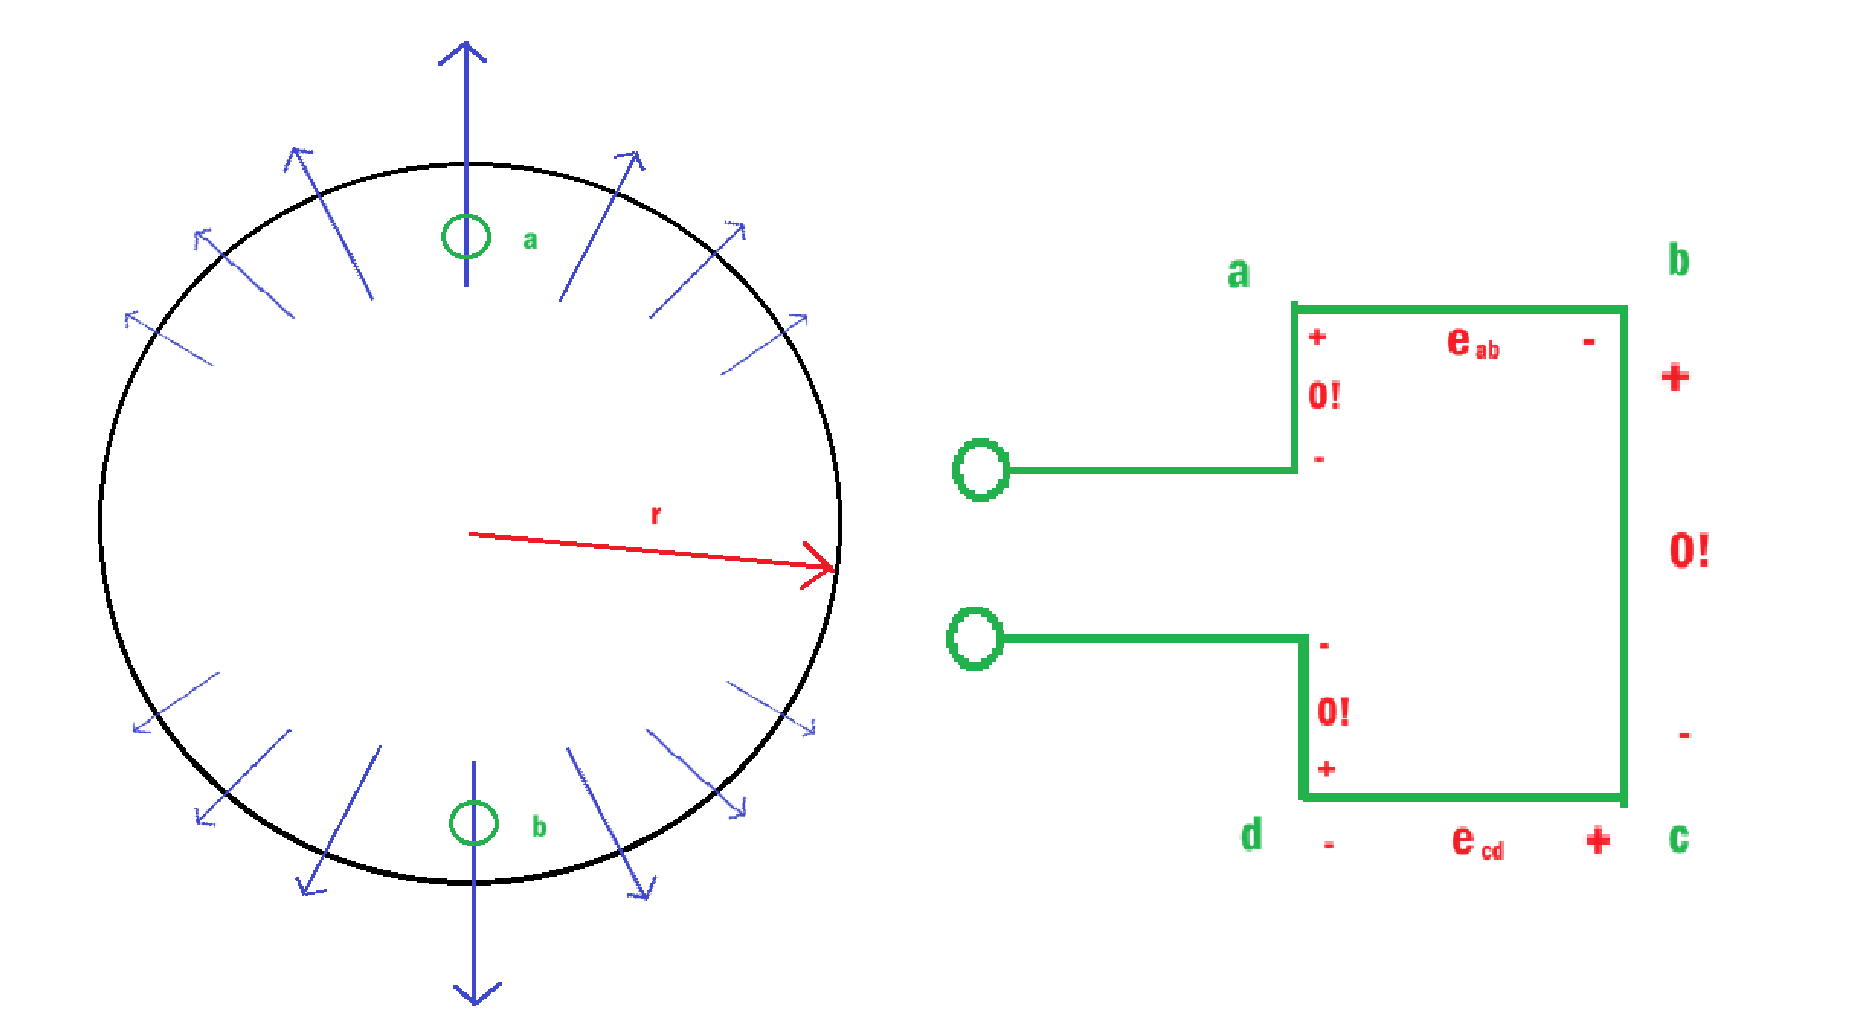
\includegraphics[width=0.6\textwidth]{assets/opstellingwikkelinggeinduceerdespanning.png}
  \caption{Opstelling}
  \label{fig:opstellingwikkelinggeinduceerdespanning.png}
 \end{figure}

Een stator­wikkeling staat stil, maar het veld draait er wel voorbij -- vanuit het
perspectief van de geleider is dat equivalent aan een geleider die door een stilstaand
veld beweegt (relatieve snelheid).
We gebruiken dus de bewegingsspanning $e = B \cdot l \cdot v_{rel}$, met
$v_{rel} = r \cdot \omega_s$ (r = straal, $\omega_s$ = synchrone snelheid), en alle
parameters hier loodrecht op elkaar.

Voor geleider $ab$ (op positie $\alpha = 0$, het draaiveld draait tegenwijzerzin trouwens
en we gaan van een poolpaar $p=1$ uit) geldt:
\begin{align*}
    e_{ab} = B \cdot |ab| \cdot v_{rel} = \hat{B}\cos(\omega_s t - p\alpha) \cdot |ab| \cdot r\omega_s = \hat{B} \cdot |ab| \cdot r\omega_s \cdot \cos(\omega_s t)
\end{align*}
De diametraal tegenoverliggende geleider $c$-$d$ zit een halve omwenteling verder
($\alpha \to \alpha - \pi$), maar door de supplementaire hoek levert dit exact dezelfde
bijdrage, hij beweegt in de andere richting:
\begin{align*}
    e_{cd} = - \hat{B} \cdot |ab| \cdot r\omega_s \cdot \cos(\omega_s t - 1 \cdot \pi) = \hat{B} \cdot |ab| \cdot r\omega_s \cdot \cos(\omega_s t)
\end{align*}
De zijdes $e_{ad}$ en $e_{bc}$ leveren geen bijdrage, want ze bewegen parallel aan het
veld.

De andere zijden van de spoel die we dus net bepaald hebben liggen in serie en versterken
elkaar, dus voor \'e\'en winding:
\begin{align*}
    e_{ab-cd} = e_{tot} = 2\hat{B}|ab| \cdot r\omega_s \cos(\omega_s t)
\end{align*}
Met $N$ windingen en de flux per winding $\hat{\Phi}$ (die de $2\hat{B}|ab|r$-term
bundelt) wordt dit:
\begin{align*}
    \boxed{e_a = N \hat{\Phi} \, \omega_s \cos(\omega_s t)}
\end{align*}

De drie fasewikkelingen liggen elk $120°$ uit elkaar rond de omtrek, wat zich vertaalt
naar een elektrische faseverschuiving in de tijd:
\begin{align*}
    e_a &= N \hat{\Phi} \, \omega_s \cos(\omega_s t) \\
    e_b &= N \hat{\Phi} \, \omega_s \cos(\omega_s t - 120°) \\
    e_c &= N \hat{\Phi} \, \omega_s \cos(\omega_s t - 240°)
\end{align*}
Let op:
dit is de \textbf{elektrische} hoek, niet de geometrische -- bij $p$ poolparen is de
elektrische hoek $p$ keer de geometrische hoek, het hoedje op de flux, betekent dat het
gaat om de piek waarde.

De effectieve (RMS) waarde volgt uit de amplitude gedeeld door $\sqrt{2}$ (met
$\omega_s = 2\pi f$):
\begin{align*}
    E = \frac{N\hat{\Phi}\cdot 2\pi f}{\sqrt{2}} = \boxed{\sqrt{2}\,\pi \, f \, N \, \hat{\Phi}}
\end{align*}

\newpage

\subsection{Opgewekte koppel}
{\color{red}(Komend stukje is vooral door AI laten cooken want er zijn meerdere
afleidingen hiervan gezien en ze zijn redelijk complex, heb ook geen idee of de
afleidingen te kennen zijn)}

Met de wet van Lorentz kunnen we het opgewekte koppel berekenen.

\begin{figure}[H]
  \centering
  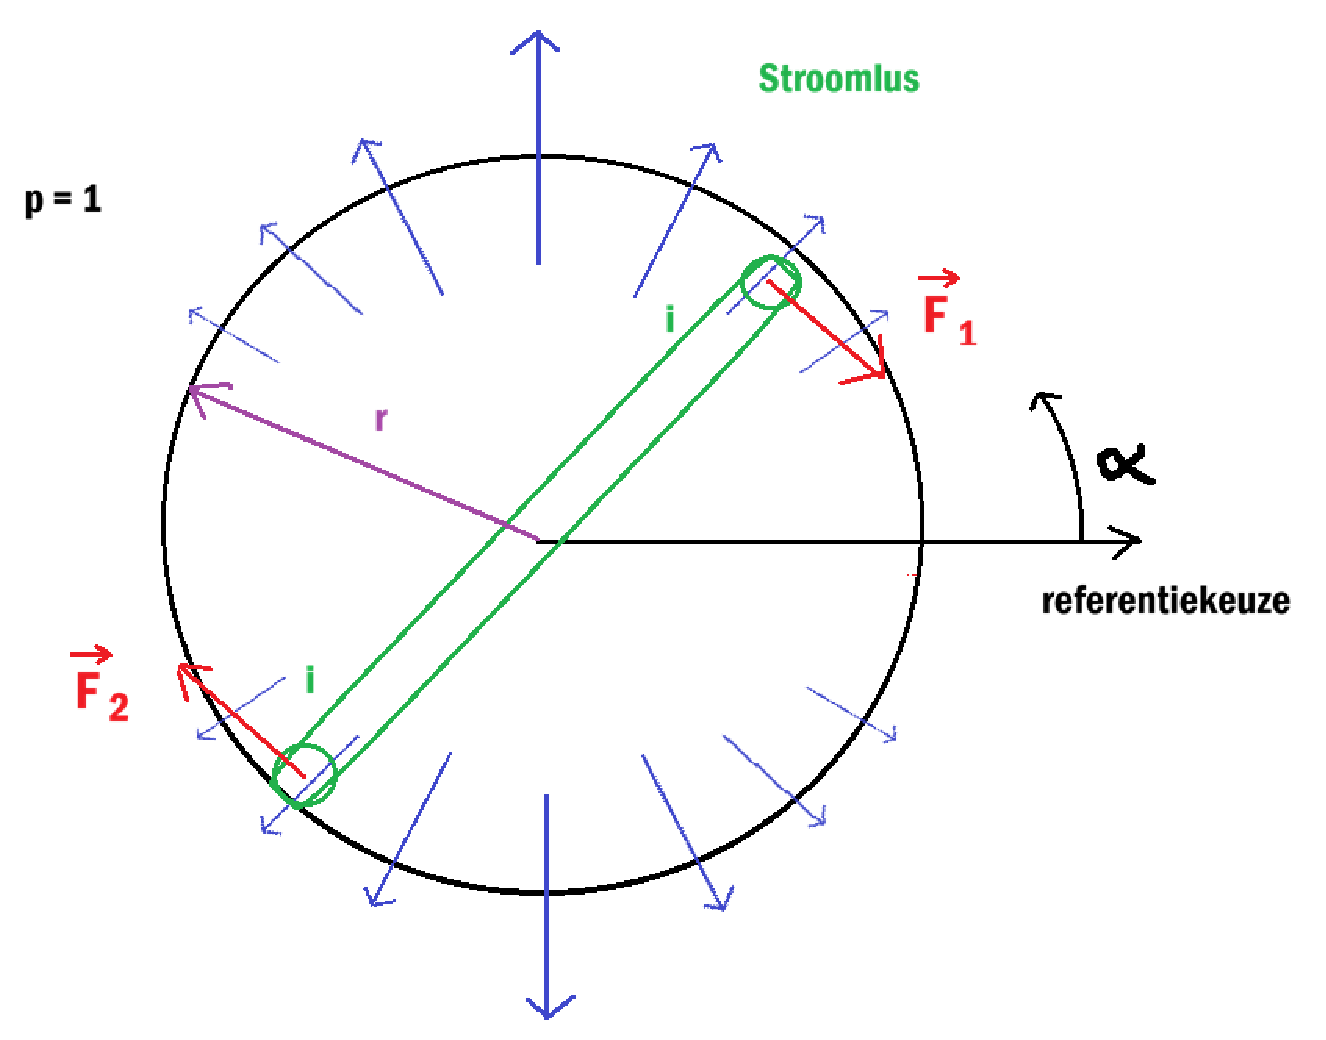
\includegraphics[width=0.5\textwidth]{assets/opstellingopgewektkoppel.png}
  \caption{Opstelling, hier is de lus onder een hoek, dit boeit in principe niet}
  \label{fig:opstellingopgewektkoppel.png}
 \end{figure}

De kracht op een geleider in een magnetisch veld is $F = B \cdot I \cdot l$, en het koppel
is $T = F \cdot r$.
Voor een rotor met $N$ geleiders en een flux $\Phi$ per poolpaar, wordt het totale koppel:
\begin{align*}
    F &= B_{\alpha} \cdot |ab| \cdot i_a \\
    &= \hat{B} \cos(\omega_s t - p\alpha) \cdot |ab| \cdot i_a
\end{align*}
Op $t=0$ (de Lorentzkracht bevat zelf geen tijdsafhankelijkheid, we bekijken dus een
momentopname) en met $p=1$ vereenvoudigt dit tot:
\begin{align*}
    F = \hat{B} \cos\alpha \cdot |ab| \cdot i_a
\end{align*}
Deze kracht werkt op beide zijden van de wikkeling (diametraal tegenover elkaar op straal
$r$), die samen een krachtenkoppel vormen.
Voor $N$ windingen wordt het totale koppel dan:
\begin{align*}
    T = N \cdot F \cdot 2r = N \cdot \hat{B}\cos\alpha \cdot |ab| \cdot i_a \cdot 2r
\end{align*}
De term $\hat{B} \cdot |ab| \cdot 2r$ is een fluxdichtheid maal een oppervlakte, en stelt
dus de piekwaarde van de flux per poolpaar voor:
$\hat{\Phi} = \hat{B}\cdot|ab|\cdot 2r$.
Zo bekomen we:
\begin{align*}
    \boxed{T = N \hat{\Phi} \cdot i_a \cdot \cos\alpha}
\end{align*}

Deze afleiding wordt verderop nog eens herhaald vanuit een net iets andere hoekreferentie
(met $\sin\alpha$ i.p.v.
$\cos\alpha$), en veralgemeend naar de vectorvorm
$\vec{T} = k \cdot \vec{B}_s \times \vec{B}_R$ -- de kernvergelijking die doorheen de rest
van de cursus terugkomt.

\subsubsection{Koppel opnieuw met Lorentz (vectorvorm)}
We herhalen de afleiding, maar nu met het statorveld t.o.v.
een andere referentie-as, en op $t=0$ (de Lorentzkracht bevat zelf geen
tijdsafhankelijkheid, we bekijken dus een momentopname):
\begin{align*}
    B_s(\alpha) = \hat{B}_s \sin\alpha
\end{align*}
De rotor draagt een stroomlus met stroom $i_R$, op straal $r$.
Elke zijde van de lus ondervindt een kracht $F_1 = N \cdot B_s(\alpha) \cdot l \cdot i_R$,
en samen vormen ze opnieuw een krachtenkoppel:
\begin{align*}
    T = F_1 \cdot 2r = N \cdot B_s(\alpha) \cdot l \cdot i_R \cdot 2r = N \cdot \hat{B}_s \sin\alpha \cdot l \cdot i_R \cdot 2r
\end{align*}
Met opnieuw $\hat{\Phi}_s = \hat{B}_s \cdot l \cdot 2r$ (piekwaarde van de statorflux):
\begin{align*}
    T = N \hat{\Phi}_s \cdot i_R \cdot \sin\alpha
\end{align*}
De rotorstroom $i_R$ wekt zelf het rotorveld $B_R$ op (wet van Ampère), dus
$i_R \propto B_R$.
Daardoor kunnen we het koppel herschrijven in termen van de twee veldgrootheden zelf:
\begin{align*}
    T = k \cdot \hat{B}_s \cdot B_R \cdot \sin\alpha
\end{align*}
met $k$ een constante.
Omdat $|\vv{B}_s \times \vv{B}_R| = B_s B_R \sin\alpha$ (met $\alpha$ de hoek tussen beide
vectoren), veralgemeent dit naar de vectorvorm:
\begin{align*}
    \boxed{\vv{T} = k \cdot \vv{B}_s \times \vv{B}_R}
\end{align*}
Dit is de kernvergelijking van draaiveldmachines:
het koppel is maximaal wanneer stator- en rotorveld loodrecht op elkaar staan
($\alpha=90°$), en nul wanneer ze uitgelijnd zijn ($\alpha=0°$) -- de rotor "probeert"
zijn veld met dat van de stator te laten samenvallen, net zoals een kompasnaald.

\newpage
